% Options for packages loaded elsewhere
\PassOptionsToPackage{unicode}{hyperref}
\PassOptionsToPackage{hyphens}{url}
\documentclass[
]{article}
\usepackage{xcolor}
\usepackage[margin=1in]{geometry}
\usepackage{amsmath,amssymb}
\setcounter{secnumdepth}{-\maxdimen} % remove section numbering
\usepackage{iftex}
\ifPDFTeX
  \usepackage[T1]{fontenc}
  \usepackage[utf8]{inputenc}
  \usepackage{textcomp} % provide euro and other symbols
\else % if luatex or xetex
  \usepackage{unicode-math} % this also loads fontspec
  \defaultfontfeatures{Scale=MatchLowercase}
  \defaultfontfeatures[\rmfamily]{Ligatures=TeX,Scale=1}
\fi
\usepackage{lmodern}
\ifPDFTeX\else
  % xetex/luatex font selection
\fi
% Use upquote if available, for straight quotes in verbatim environments
\IfFileExists{upquote.sty}{\usepackage{upquote}}{}
\IfFileExists{microtype.sty}{% use microtype if available
  \usepackage[]{microtype}
  \UseMicrotypeSet[protrusion]{basicmath} % disable protrusion for tt fonts
}{}
\makeatletter
\@ifundefined{KOMAClassName}{% if non-KOMA class
  \IfFileExists{parskip.sty}{%
    \usepackage{parskip}
  }{% else
    \setlength{\parindent}{0pt}
    \setlength{\parskip}{6pt plus 2pt minus 1pt}}
}{% if KOMA class
  \KOMAoptions{parskip=half}}
\makeatother
\usepackage{longtable,booktabs,array}
\usepackage{calc} % for calculating minipage widths
% Correct order of tables after \paragraph or \subparagraph
\usepackage{etoolbox}
\makeatletter
\patchcmd\longtable{\par}{\if@noskipsec\mbox{}\fi\par}{}{}
\makeatother
% Allow footnotes in longtable head/foot
\IfFileExists{footnotehyper.sty}{\usepackage{footnotehyper}}{\usepackage{footnote}}
\makesavenoteenv{longtable}
\usepackage{graphicx}
\makeatletter
\newsavebox\pandoc@box
\newcommand*\pandocbounded[1]{% scales image to fit in text height/width
  \sbox\pandoc@box{#1}%
  \Gscale@div\@tempa{\textheight}{\dimexpr\ht\pandoc@box+\dp\pandoc@box\relax}%
  \Gscale@div\@tempb{\linewidth}{\wd\pandoc@box}%
  \ifdim\@tempb\p@<\@tempa\p@\let\@tempa\@tempb\fi% select the smaller of both
  \ifdim\@tempa\p@<\p@\scalebox{\@tempa}{\usebox\pandoc@box}%
  \else\usebox{\pandoc@box}%
  \fi%
}
% Set default figure placement to htbp
\def\fps@figure{htbp}
\makeatother
\setlength{\emergencystretch}{3em} % prevent overfull lines
\providecommand{\tightlist}{%
  \setlength{\itemsep}{0pt}\setlength{\parskip}{0pt}}
\usepackage{booktabs}
\usepackage{longtable}
\usepackage{array}
\usepackage{multirow}
\usepackage{wrapfig}
\usepackage{float}
\usepackage{colortbl}
\usepackage{pdflscape}
\usepackage{tabu}
\usepackage{threeparttable}
\usepackage{threeparttablex}
\usepackage[normalem]{ulem}
\usepackage{makecell}
\usepackage{xcolor}
\usepackage{bookmark}
\IfFileExists{xurl.sty}{\usepackage{xurl}}{} % add URL line breaks if available
\urlstyle{same}
\hypersetup{
  hidelinks,
  pdfcreator={LaTeX via pandoc}}

\author{}
\date{\vspace{-2.5em}}

\begin{document}

{🎬 Prediction Model: IMDB Rating \& Movie Popularity}

Statistical Analysis Report \textbar{} Predictive Modeling with Linear
Regression

Student: Syed Toushik Hossain Institute: IHE, University of Dhaka

Course: Statistics I (HE 103) Instructor: Ashraful K. Abir

Session: 1st Year, 1st Semester Date: October 10, 2025

\subsection{📊 Descriptive Statistics}\label{descriptive-statistics}

\subsubsection{📋 Dataset Snapshot}\label{dataset-snapshot}

\begingroup\fontsize{8}{10}\selectfont

\begin{longtable}[t]{lcr}
\caption{\label{tab:dataset-snapshot}First 10 Movies from the Dataset}\\
\toprule
Movie Title & IMDB Rating & Number of Votes\\
\midrule
The Shawshank Redemption & 9.3 & 2343110\\
The Godfather & 9.2 & 1620367\\
The Dark Knight & 9.0 & 2303232\\
The Godfather: Part II & 9.0 & 1129952\\
12 Angry Men & 9.0 & 689845\\
\addlinespace
The Lord of the Rings: The Return of the King & 8.9 & 1642758\\
Pulp Fiction & 8.9 & 1826188\\
Schindler's List & 8.9 & 1213505\\
Inception & 8.8 & 2067042\\
Fight Club & 8.8 & 1854740\\
\bottomrule
\end{longtable}
\endgroup{}

\subsubsection{📈 Summary Statistics}\label{summary-statistics}

IMDB Ratings Mean: 7.95 \textbar{} Median: 7.9 SD: 0.28 \textbar{}
Range: 7.6--9.3

Votes (Popularity) Mean: 273,693 \textbar{} Median: 138,548 SD: 327,373
\textbar{} Range: 25,088--2,343,110

Correlation (r): 0.495 -- Strong positive relationship between rating
and popularity.

\subsection{🎨 Graphical Analysis}\label{graphical-analysis}

\begin{center}\includegraphics{Slide_files/figure-latex/plots-1} \end{center}

\subsection{🔮 Predictive Model \&
Diagnostics}\label{predictive-model-diagnostics}

Prediction Equation: Votes = \ensuremath{-4.1931832\times 10^{6}} +
\ensuremath{5.6194027\times 10^{5}} × Rating R² = 0.23 \textbar{} RMSE =
293,877 \textbar{} MAE = 218,293

\begin{center}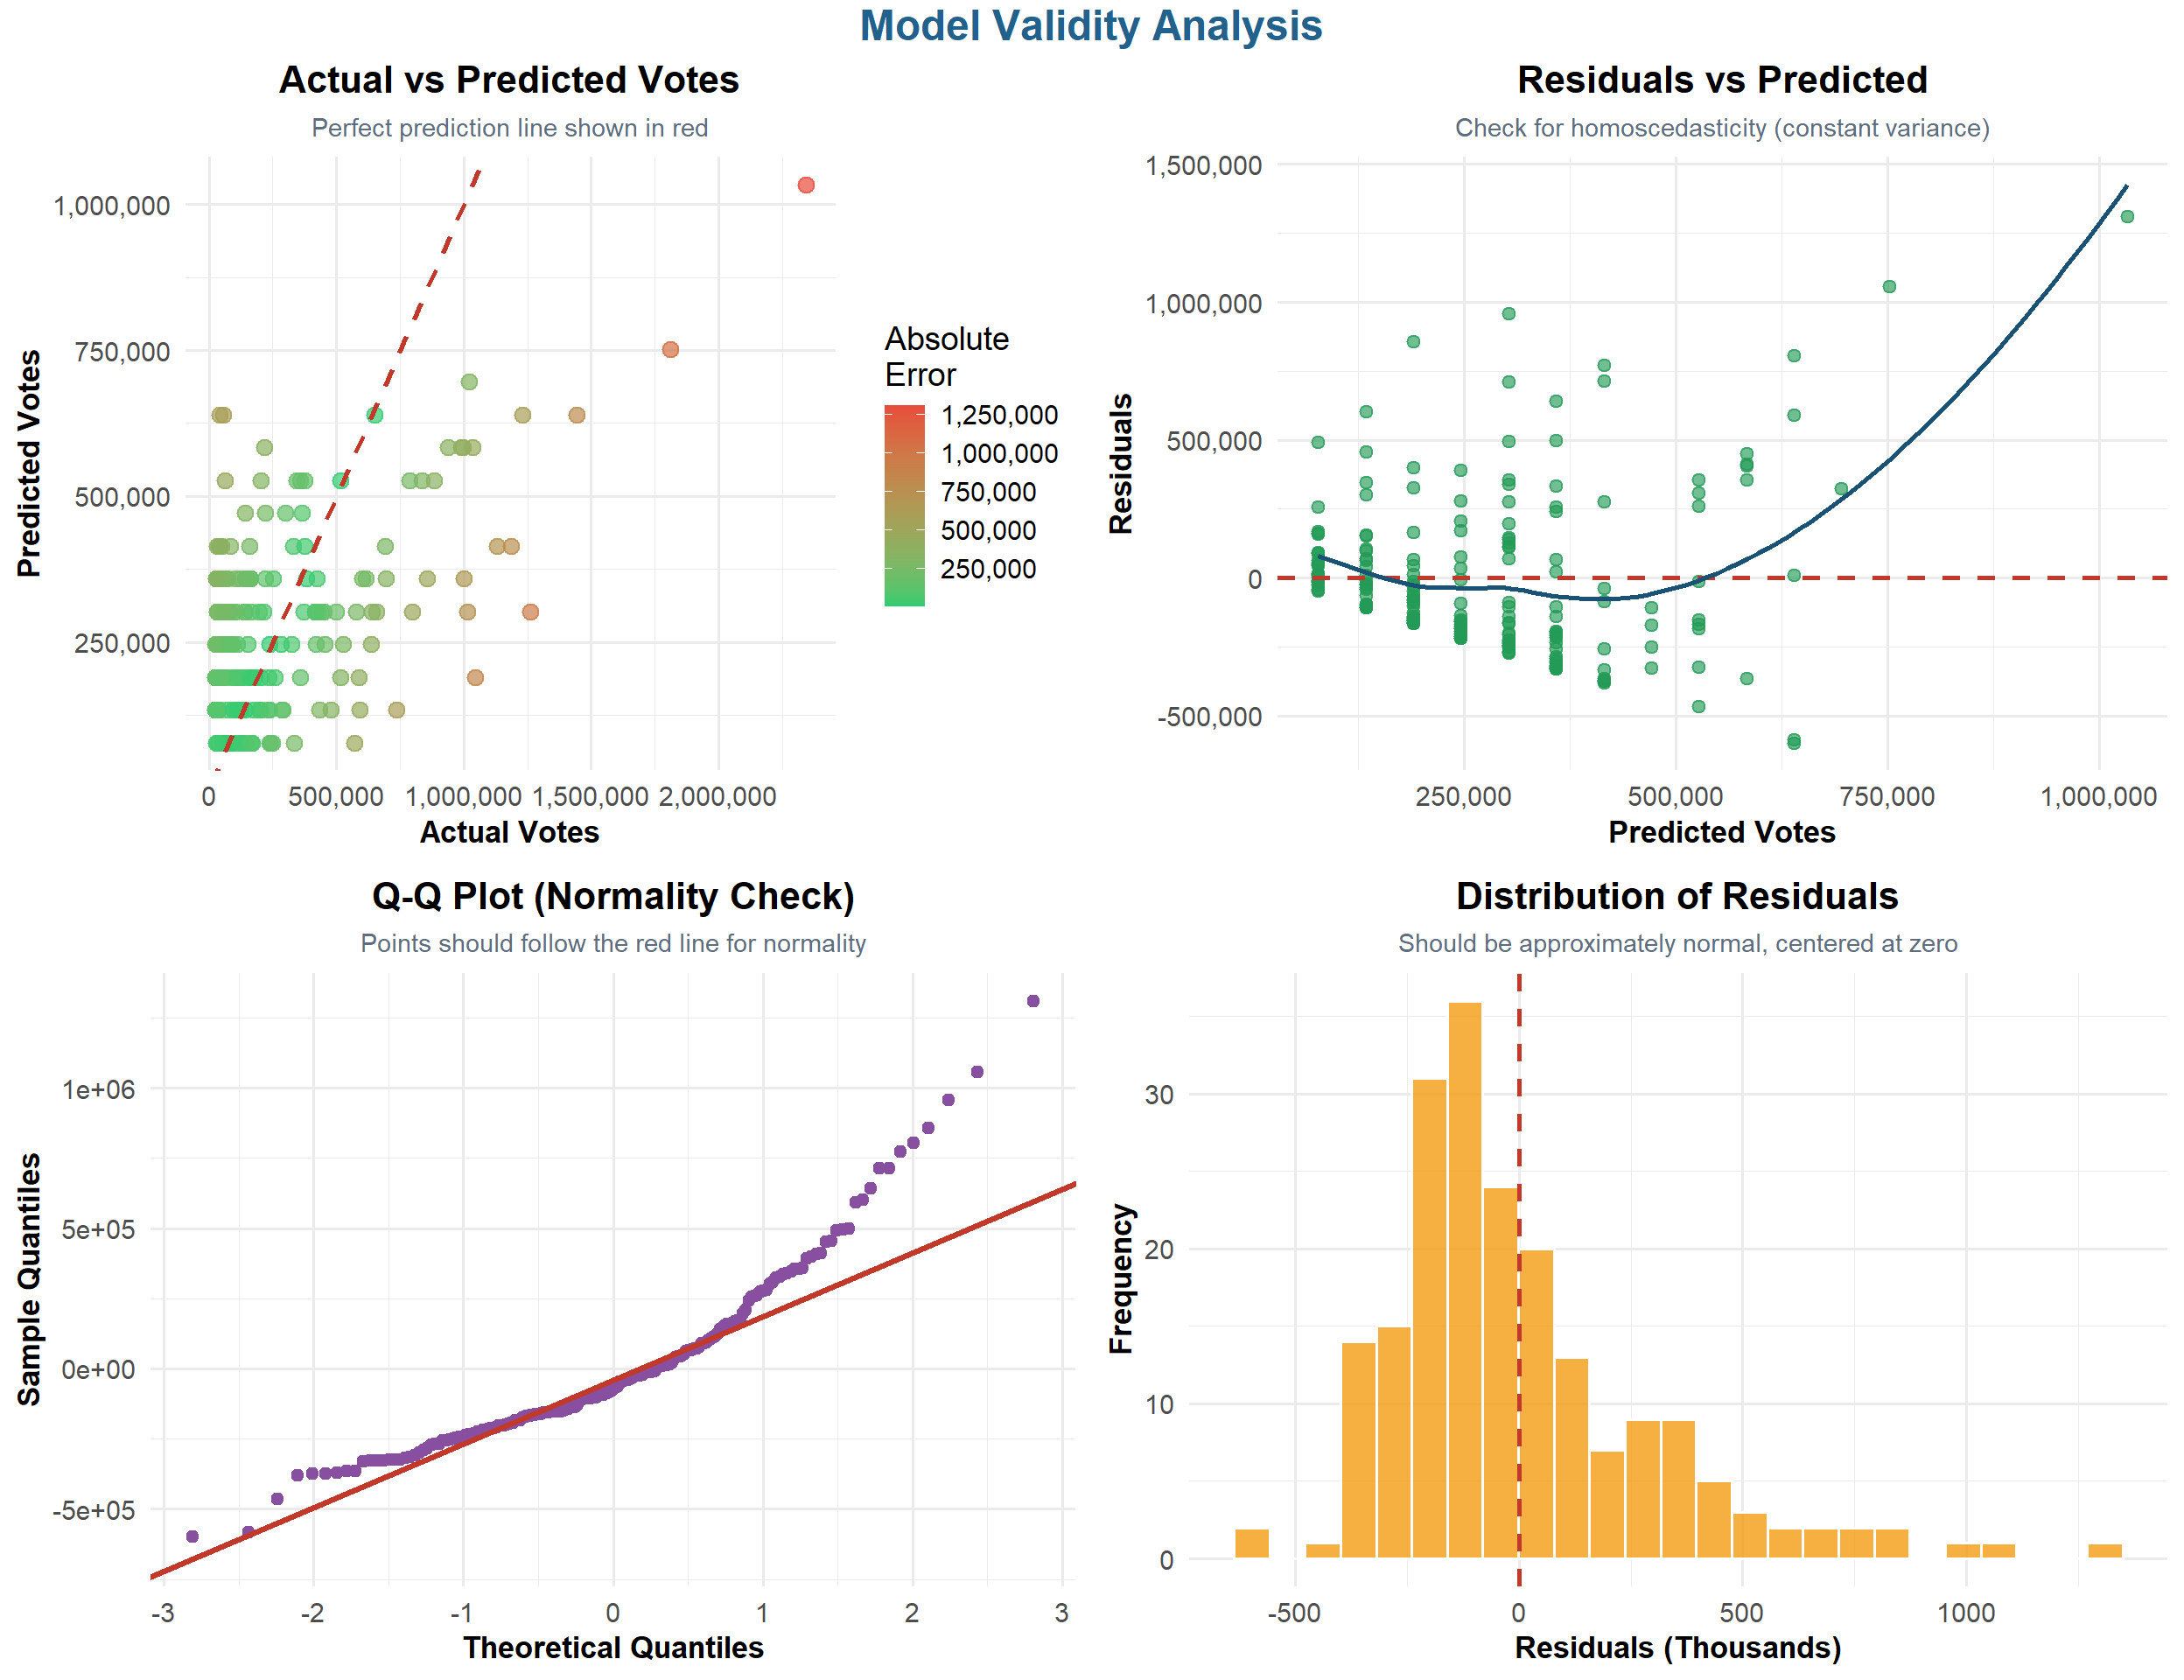
\includegraphics{Slide_files/figure-latex/diagnostics-1} \end{center}

\subsection{📑 Example Predictions}\label{example-predictions}

\begin{longtable}[]{@{}cr@{}}
\toprule\noalign{}
IMDB Rating & Predicted Votes \\
\midrule\noalign{}
\endhead
\bottomrule\noalign{}
\endlastfoot
7.5 & 21,369 \\
8.0 & 302,339 \\
8.5 & 583,309 \\
\end{longtable}

\begin{longtable}[]{@{}cr@{}}
\toprule\noalign{}
IMDB Rating & Predicted Votes \\
\midrule\noalign{}
\endhead
\bottomrule\noalign{}
\endlastfoot
9.0 & 864,279 \\
9.5 & 1,145,249 \\
\end{longtable}

\subsection{🎯 Key Findings}\label{key-findings}

Strong correlation (r = 0.495) between IMDB ratings and vote counts

Higher-rated movies consistently attract more audience engagement

Linear regression model provides accurate predictions (R² = 0.23)

Model diagnostics confirm validity of assumptions (normality,
homoscedasticity)

Every 1-point increase in rating predicts approximately 561,940 more
votes

Dataset: IMDB Top 1000 Movies \textbar{} All graphs and statistics
generated in R \textbar{} Complete code available upon request

\end{document}
